%%%%%%%%%%%%%%%%%%%%%%%%%%%%%%%%%%%%%%%%%
% Short Sectioned Assignment
% LaTeX Template
% Version 1.0 (5/5/12)
%
% This template has been downloaded from:
% http://www.LaTeXTemplates.com
%
% Original author:
% Frits Wenneker (http://www.howtotex.com)
%
% License:
% CC BY-NC-SA 3.0 (http://creativecommons.org/licenses/by-nc-sa/3.0/)
%
%%%%%%%%%%%%%%%%%%%%%%%%%%%%%%%%%%%%%%%%%

%----------------------------------------------------------------------------------------
%	PACKAGES AND OTHER DOCUMENT CONFIGURATIONS
%----------------------------------------------------------------------------------------

\documentclass[paper=a4, fontsize=11pt]{scrartcl} % A4 paper and 11pt font size
\usepackage{amsmath,amsfonts,graphicx}
\usepackage{lastpage}	% Required to determine the last page for the footer
\usepackage{booktabs}
%\usepackage{algpseudocode}
\usepackage{tikz}
\usepackage{algorithm}
\usepackage{algorithmicx}
\usepackage{algpseudocode}
\usepackage[top=2cm, bottom=2cm, left=2cm, right=2cm]{geometry}

\usepackage{listings}
\usepackage{color}
\usepackage{xcolor}
\definecolor{dkgreen}{rgb}{0,0.6,0}
\definecolor{gray}{rgb}{0.5,0.5,0.5}
\definecolor{mauve}{rgb}{0.58,0,0.82}
\lstset{frame=tb,
     %language=Java,
     aboveskip=3mm,
     belowskip=3mm,
     showstringspaces=false,
     columns=flexible,
     basicstyle = \ttfamily\small,
     numbers=none,
     numberstyle=\tiny\color{gray},
     keywordstyle=\color{blue},
     commentstyle=\color{dkgreen},
     stringstyle=\color{mauve},
     breaklines=true,
     breakatwhitespace=true,
     tabsize=3
}

%\usepackage[]{algorithm2e}

\usepackage[T1]{fontenc} % Use 8-bit encoding that has 256 glyphs
\usepackage{fourier} % Use the Adobe Utopia font for the document - comment this line to return to the LaTeX default
\usepackage[english]{babel} % English language/hyphenation
\usepackage{amsmath,amsfonts,amsthm} % Math packages

\usepackage{lipsum} % Used for inserting dummy 'Lorem ipsum' text into the template

\usepackage{sectsty} % Allows customizing section commands
\allsectionsfont{\centering \normalfont\scshape} % Make all sections centered, the default font and small caps

\usepackage{fancyhdr} % Custom headers and footers
    \pagestyle{fancyplain} % Makes all pages in the document conform to the custom headers and footers
    \fancyhead[L]{\textsc{COMP90007 Assignment 2}}
    \fancyhead[R]{\textsc{Student Number: 955986 Username:} peiyongw} % No page header - if you want one, create it in the same way as the footers below
    \fancyfoot[L]{} % Empty left footer
    \fancyfoot[C]{} % Empty center footer
    \fancyfoot[R]{\textsc{Page} \thepage \textsc{ of} \pageref{LastPage}} % Page numbering for right footer
    \renewcommand{\headrulewidth}{0pt} % Remove header underlines
    \renewcommand{\footrulewidth}{0pt} % Remove footer underlines
    \setlength{\headheight}{13.6pt} % Customize the height of the header

\numberwithin{equation}{section} % Number equations within sections (i.e. 1.1, 1.2, 2.1, 2.2 instead of 1, 2, 3, 4)
\numberwithin{figure}{section} % Number figures within sections (i.e. 1.1, 1.2, 2.1, 2.2 instead of 1, 2, 3, 4)
\numberwithin{table}{section} % Number tables within sections (i.e. 1.1, 1.2, 2.1, 2.2 instead of 1, 2, 3, 4)

\setlength\parindent{0pt} % Removes all indentation from paragraphs - comment this line for an assignment with lots of text

%----------------------------------------------------------------------------------------
%	TITLE SECTION
%----------------------------------------------------------------------------------------

\newcommand{\horrule}[1]{\rule{\linewidth}{#1}} % Create horizontal rule command with 1 argument of height

\title{	
\normalfont \normalsize 
\textsc{The University of Melbourne } \\ [25pt] % Your university, school and/or department name(s)
\horrule{0.5pt} \\[0.4cm] % Thin top horizontal rule
\huge COMP90007 Internet Technologies SM2, 2018
Assignment 2 \\ % The assignment title
\horrule{2pt} \\[0.5cm] % Thick bottom horizontal rule
}

\author{Peiyong Wang $\,$ 955986 (username:peiyongw)} % Your name

\date{\normalsize\today} % Today's date or a custom date

\begin{document}

\maketitle % Print the title
\thispagestyle{empty}%no head or foot on the first page


\section{Question One}
Since CB = 5, CD = 4, CE = 3, to reach A, we have:
$$CBA = 5+5=10$$
$$CDA=4+15=20$$
$$CEA=3+8=11$$
$$CBF=5+4=9$$
$$CDF=4+4=8$$
$$CEF=3+6=9$$
So to reach A, the transmission will go through B first; and to get to F, the 
transmission will go thtough D first.



The expected delay and the outgoing line of C are shown as follows (Table 1.1):

\begin{table}[htbp]
    \centering
    \caption{Expected delay and outgoing line of C}
    \begin{tabular}{ccc}
    \hline
    To &Delay & Line \\
    \hline
    A&10&B\\
    B&5&B\\
    C&0&-\\
    D&4&D\\
    E&3&E\\
    F&8&D\\
    \hline
    \end{tabular}
\end{table}

Then we can have C's routing table as follows (Table 1.2):

\begin{table}[htbp]
    \centering
    \caption{Routing table of C}
    \begin{tabular}{cc}
        \hline
        Dest.&Line\\
        \hline
        A&B\\
        B&B\\
        C&-\\
        D&D\\
        E&E\\
        F&D\\
        \hline
    \end{tabular}
\end{table}
And the updated routing vectors for B, D, E repectively (Table 1.3):
\begin{table}[htbp]
    \centering
    \caption{Routing vectors for B, D and E}
    \begin{tabular}{cccc}
        \hline
        Dest.&B&D&E \\
        \hline
        A&10&19&11\\
        B&5&17&8\\
        C&14&11&7\\
        D&16&4&12\\
        E&12&12&3\\
        F&9&8&9\\
        \hline
    \end{tabular}
\end{table}
\newpage
\section{Question Two}
\paragraph{a}
Convert 255.255.240.0 to binary we can have 11111111.11111111.11110000.00000000, there are 16 network bits and 4 bits  for subnets,
 so the number of subnets allowed is 
$2^{4}=16$

\paragraph{b} 
Firstly, we round up the number of addresses to 2048, 1024, 2048, 2048 repectively.
For A, since $2048 = 2^{11}$, so we can see that it need 11 bits for hosts. For there are already
8 bits in the last part of the IP address, the hosts from A will only need the last three bits of 
the third part of the IP address, then the ending address of A will be 128.16.7.255, and the subnet
mask will be 128.16.8.0/21. It goes the same for B. 

However, when it comes to C, the original 3 bits of the third part of the IP address is not enough,
so the C will start from the first one of the last four bits, hence 00001000. The rest calculation part is
the same as A. So we can have C starting from 128.16.16.0 and ending at 128.16.23.255 with mask 128.16.16.0/21.
The calculation process for D is the same as C. Results see Table 2.1.
\begin{table}[htbp]
    \centering
    \caption{Answer for question 2B}
    \begin{tabular}{ccccc}
        \hline
        Organisation&Starting Add&Ending Add&Adds Allocated&Mask \\
        \hline
        A&128.16.0.0&128.16.7.255&2048&128.16.0.0/21\\
        B&128.16.8.0&128.16.11.255&1024&128.16.8.0/22\\
        C&128.16.16.0&128.16.23.255&2048&128.16.16.0/21\\
        D&128.16.32.0&128.16.47.255&4096&128.16.32.0/20\\
        \hline
    \end{tabular}
\end{table}

\section{ Question Three}
According to Carrier Sense Multiple Access Protocol, when station C wants to 
transmit to station B, it will send a small impulse of signal to check whether
there is any other signal currently occupying the channel. 

\vbox{  }
Since C detects no collision, which means currently no one else is transmitting messages.

\vbox{  }
However, when the propagation delay is extremely high, in such a case even other stations
have sent out a transmission (which have not reached its destination yet since the high delay)
 C can still reach the conclusion that currently the channel is idle. So when C send out a 
 transmission, it will collide with others.

 \vbox{ }
 Therefore we can conclude that there is a possibility that B will not recieve the transmission
  from C.

\vbox{ }
However, when using  Multiple Access with Collision Avoidance Protocol, things can
be different. The MACA requires sender C send a RTS to reciever B, and the data transmission will
not commence until B replies with a CTS.

\vbox{ }
For other stations sharing the same channel, when they detect RTS or CTS they will remian silent until
the data transmission process is complete. So in the MACA case the transmission will be successful.

\section{Question Four}
\paragraph{a} To make it easier to distinguish valid frames from garbage.
\paragraph{b} When transmitted by Ethernet, the minimum length of Ethernet frame is 
64 bytes, including the destination address and the source address, the type/length field,
and the checksum, summing up to 18 bytes. Plus the 62-byte packet, the total 
length of the frame is 80 bytes, which exceeds the minimum length of 64 bytes. Hence
there is no need for padding. 
%\newpage
\section{Question Five}
11 slots are needed to resolve the contention.


\begin{figure}[htbp]
    \centering
    
    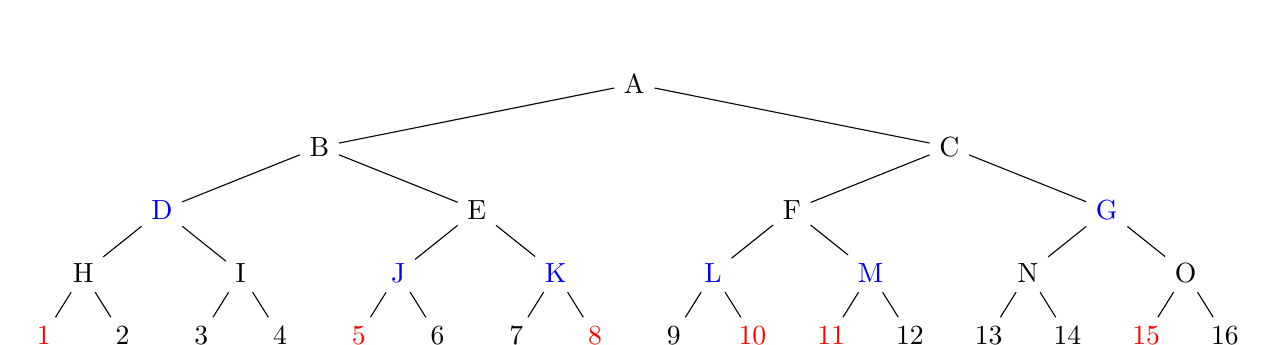
\begin{tikzpicture}
        [level distance=1.3cm,
    level 1/.style={sibling distance=8cm, level distance=0.8cm},
    level 2/.style={sibling distance=4cm, level distance=0.8cm},
    level 3/.style={sibling distance=2cm, level distance=0.8cm},
    level 4/.style={sibling distance=1cm, level distance=0.8cm}]
    \node {A}
    child{node{B}
        child{node{\color{blue}D}
            child{node{H}
                child{node{\color{red}1}}
                child{node{2}}}
            child{node{I}
                child{node{3}}
                child{node{4}}}}
        child{node{E}
            child{node{\color{blue}J}
                child{node{\color{red}5}}
                child{node{6}}}
            child{node{\color{blue}K}
                child{node{7}}
                child{node{\color{red}8}}}}}
    child{node{C}
        child{node{F}
            child{node{\color{blue}L}
                child{node{9}}
                child{node{\color{red}10}}}
            child{node{\color{blue}M}
                child{node{\color{red}11}}
                child{node{12}}}}
        child{node{\color{blue}G}
            child{node{N}
                child{node{13}}
                child{node{14}}}
            child{node{O}
                child{node{\color{red}15}}
                child{node{16}}}}}
    ;
    
    \end{tikzpicture}
    \caption{Adaptive tree walk protocol for solving contention. Red digits are stations which are ready,
    blue characters are the nodes where the contention is resolved.}
\end{figure}
\textsc{Slot 1: } 1,5,8,10,11,15;(Node A)

\textsc{Slot 2: }  1,5,8;(Node B)

\textsc{Slot 3: }  1;(Node D)

\textsc{Slot 4: }  5,8;(Node E)

\textsc{Slot 5: }  5;(Node J)

\textsc{Slot 6: }  8;(Node K)

\textsc{Slot 7: }  10,11,15;(Node C)

\textsc{Slot 8: }  10,11;(Node F)

\textsc{Slot 9:  }  10;(Node L)

\textsc{Slot 10:} 11;(Node M)

\textsc{Slot 11:} 15.(Node G)



\end{document}



%\begin{align} 
%\begin{split}
%(x+y)^3 	&= (x+y)^2(x+y)\\
%&=(x^2+2xy+y^2)(x+y)\\
%&=(x^3+2x^2y+xy^2) + (x^2y+2xy^2+y^3)\\
%&=x^3+3x^2y+3xy^2+y^3
%\end{split}					
%\end{align}





%\begin{tabbing}
%\hspace*{.25in} \= \hspace*{.25in} \= \hspace*{.25in} \= \hspace*{.25in} \= \hspace*{.25in} \=\kill
%\>$Euclid(m,n)=$ \\
%\>\> {\bf while} n$ \neq $ 0 \\
%\>\>\> r $ \leftarrow $ $m$ mod $n$  \\
%\>\>\>  m $\leftarrow$n\\
%\>\>{\bf return} m 
%\end{tabbing}

%Python code:
%\begin{lstlisting}[language = python]
%def gcd(m,n):
%	while n != 0:
%		r = m % n
%		m = n
%		n = r
%	return m
%\end{lstlisting}


%\paragraph{Heading on level 4 (paragraph)}




%\begin{tabbing}
%	\hspace*{.25in} \= \hspace*{.25in} \= \hspace*{.25in} \= \hspace*{.25in} \= \hspace*{.25in} \=\kill
%	{\bf function} find (A,x,n)\\
%	\> j $\leftarrow$ 0\\
%	\> {\bf while} j < n\\
%	\>\> {\bf if} A[j]=x\\
%	\>\>\>  {\bf return} j  \\
%	\>\> j $\leftarrow$ j+1\\
%	\> {\bf return} -1
%\end{tabbing}


%\begin{figure}[htbp!]
%		\centering
%		\includegraphics[width=0.6\textwidth]{lec26.png}
%		\caption{Linked List}%\label{book}
%		\vspace{-1em}
%\end{figure}






%\begin{align}
%A = 
%\begin{bmatrix}
%A_{11} & A_{21} \\
%A_{21} & A_{22}
%\end{bmatrix}
%\end{align}



%\begin{algorithm}
 %       \caption{Count the number of occurrences of a certain integer $x$ in an array $A[]$}
  %      \begin{algorithmic}[1] %每行显示行号
   %         \Require  $Array$ A[],$Length\;of\;the\;array$ n, $Integer$ x
    %        \Ensure   Number of occurrence of integer x  
     %       \Function {NumberCount}{$A[], x,n$}
      %      
       %     	\State $firstApperence \gets $\Call{FirstOccurrenceSearch}{$A[]$,0,$n-1$,$x$,$n$}
            	
        %    	\If{$firstApperence=-1$}
         %   	\State \Return $firstApperence$
          %  	\EndIf
            	
           % 	\State $lastApperence\gets$ \Call{LastOccurrenceSearch}{$A[],firstApperence,n-1,x,n$}
            %	\State \Return $lastApperence-firstApperence+1$
            	
                %\State $result \gets 0$
                
                %\If {$high \geqslant low$}
                    %\State $mid \gets (high + low) // 2$   \#"//" means integer division
                    %\State $result \gets result +$ \Call{MergerSort}{$Array, left, middle$}
                    %\State $result \gets result +$ \Call{MergerSort}{$Array, middle, right$}
                    %\State $result \gets result +$ \Call{Merger}{$Array,left,middle,right$}
                %\EndIf
                %\If {$mid = 0 \, OR x > A[mid-1]$}
                %	\State \Return $mid$
                %\Else 
                %	\If {$x>A[mid]$}
                %		\State \Return 
                
                 %\Return{$result$}
            %\EndFunction
           %\State
            %\Function{FirstOccurrenceSearch}{$A[],low, high,x,n$}
            
      %      \If{$high \geqslant low$}
      %      \State $mid\gets(low + high)//2$ \Comment "//" means integer division
      %      \EndIf
      %      \If{$\{mid = 0 \; OR\;  x>A[mid-1]\}\; AND\; \{A[mid]=x\}$} 
      %      \State \Return $mid$
      %      \Else
      %      	\If{$x>A[mid]$}
      %      	\State \Return \Call{FirstOccurrenceSearch}{$A[],mid+1,high,x,n$}
      %      	\Else
      %      	\State \Return \Call{FirstOccurrenceSearch}{$A[],low,mid-1,x,n$}
      %      	\EndIf
      %      \EndIf
      %      \State \Return -1
      %      
      %      \EndFunction
      %      
      %      \State
      %      \Function{LastOccurrenceSearch}{$A[],low,high,x,n$}
      %      
      %      \If{$high \geqslant low$}
      %      \State $mid\gets(low + high)//2$ \Comment "//" means integer division
      %      \EndIf
      %      \If{$\{mid = n-1 \; OR\;  x<A[mid-1]\}\; AND\; \{A[mid]=x\}$} 
      %      \State \Return $mid$
      %     \Else
       %     	\If{$x<A[mid]$}
        %    	\State \Return \Call{LastOccurrenceSearch}{$A[],low, mid-1, x,n$}
         %   	\Else
          %  	\State \Return \Call{LastOccurrenceSearch}{$A[],mid+1, high,x,n$}
           % 	\EndIf
            %\EndIf
            %\State \Return -1
            
            

           % \EndFunction
            
            %\Function{Merger}{$Array, left, middle, right$}
             %   \State $i\gets left$
              %  \State $j\gets middle$
               % \State $k\gets 0$
               % \State $result \gets 0$
               % \While{$i<middle$ \textbf{and} $j<right$}
                %    \If{$Array[i]<Array[j]$}
                 %       \State $B[k++]\gets Array[i++]$
                  %  \Else
                   %     \State $B[k++] \gets Array[j++]$
                    %    \State $result \gets result + (middle - i)$
                    %\EndIf
                %\EndWhile
                %\While{$i<middle$}
                %    \State $B[k++] \gets Array[i++]$
                %\EndWhile
                %\While{$j<right$}
                %    \State $B[k++] \gets Array[j++]$
                %\EndWhile
                %\For{$i = 0 \to k-1$}
                %    \State $Array[left + i] \gets B[i]$
                %\EndFor
                %\State \Return{$result$}
            %\EndFunction
      %  \end{algorithmic}
    %\end{algorithm}





